% libgomo developer and contributor guide.
% Build (out of tree): latexmk -pdf -outdir=<dir> docs/guide/developer-guide.tex
\documentclass[11pt,a4paper]{article}

\usepackage[T1]{fontenc}
\usepackage[utf8]{inputenc}
\usepackage{lmodern}
\usepackage[margin=2.3cm]{geometry}
\usepackage{microtype}
\usepackage{xcolor}
\usepackage{listings}
\usepackage{booktabs}
\usepackage{tabularx}
\usepackage{array}
\usepackage{enumitem}
\usepackage{tikz}
\usetikzlibrary{arrows.meta,positioning,fit,calc}
\usepackage[hidelinks]{hyperref}

\definecolor{codebg}{HTML}{F6F8FA}
\definecolor{kw}{HTML}{0033B3}
\definecolor{cm}{HTML}{6A737D}
\definecolor{st}{HTML}{067D17}

% One style for the three figures. Fill shade marks the layer; every box also names its module,
% so no meaning rests on colour alone. Dotted boxes are outside libgomo.
\colorlet{layercore}{gray!20}
\colorlet{layeradapter}{blue!10}
\colorlet{layerio}{green!12}
\colorlet{layerhelper}{orange!15}
\tikzset{
  pg figure/.style={font=\small, line width=0.6pt},
  pg arrow/.style={-{Stealth[length=2mm]}, line width=0.8pt},
  pg mod/.style={draw, rounded corners=2pt, minimum width=2.3cm, minimum height=0.75cm,
                 font=\small\ttfamily, fill=#1},
  pg mod/.default={white},
  pg ext/.style={draw, dotted, rounded corners=2pt, minimum width=2.3cm, minimum height=0.75cm,
                 font=\small\itshape, fill=white},
  pg group/.style={draw, dashed, rounded corners=4pt, inner sep=6pt},
  pg note/.style={font=\scriptsize\itshape, align=center},
  pg label/.style={font=\scriptsize\ttfamily, fill=white, inner sep=1pt},
  pg lifeline/.style={dashed, black!45}}

\lstdefinestyle{cpp}{
  language=C++, basicstyle=\ttfamily\footnotesize, backgroundcolor=\color{codebg},
  keywordstyle=\color{kw}\bfseries, commentstyle=\color{cm}\itshape, stringstyle=\color{st},
  morekeywords={constexpr,override,final,noexcept,nullptr,auto,using},
  columns=fullflexible, keepspaces=true, showstringspaces=false, breaklines=true,
  frame=single, rulecolor=\color{black!15}, xleftmargin=4pt, xrightmargin=4pt,
  aboveskip=8pt, belowskip=8pt, upquote=true}
\lstdefinestyle{sh}{
  basicstyle=\ttfamily\footnotesize, backgroundcolor=\color{codebg}, columns=fullflexible,
  keepspaces=true, showstringspaces=false, breaklines=true, frame=single,
  rulecolor=\color{black!15}, xleftmargin=4pt, xrightmargin=4pt, upquote=true}
\lstset{style=cpp}

\newcommand{\code}[1]{\texttt{#1}}
\newcommand{\file}[1]{\texttt{#1}}

\setlist{itemsep=2pt,topsep=4pt}
\setlength{\parskip}{4pt}
\setlength{\emergencystretch}{3em}

\title{\textbf{libgomo}\\[4pt]\large Developer and Contributor Guide}
\author{libgomo project}
\date{Version 0.1.0 \quad--\quad November 2026}

\begin{document}
\maketitle

\begin{abstract}
\noindent libgomo is a C++23 framework that connects applications to Gomoku engines. An application
talks to one protocol-neutral interface, \code{EnginePort}; adapters translate it to the wire
protocol an engine speaks (Gomocup, also called Piskvork, with Yixin extensions; GTP with KataGomo
extensions; and KataGomo's \code{gom} mode) and parse the engine's text output into typed events.
This guide starts with a first search, explains the architecture, gives step-by-step guides for
using and extending the library, collects the reference facts, and describes how to contribute.
\end{abstract}

\tableofcontents
\newpage


%######################################################################
\part{Getting started}
%######################################################################

%======================================================================
\section{Overview}
%======================================================================

\subsection{What libgomo does}

libgomo is the protocol layer between an application (a GUI, a match runner, an analysis tool) and
a Gomoku engine running as a separate process. Its priorities, in order:

\begin{enumerate}
  \item \textbf{Low coupling.} The application never sees protocol text. The core knows no
        protocol, no process and no I/O.
  \item \textbf{Multiple protocols.} One interface over several wire protocols.
  \item \textbf{Open for extension.} A new protocol is a new adapter; the core and existing
        adapters do not change (open--closed and dependency-inversion principles).
  \item \textbf{Tolerant parsing.} Engine output varies from terse to detailed. Parsers are pure
        and total: a line they do not understand is kept as an \code{UnparsedEvent}, never dropped.
\end{enumerate}

\noindent Out of scope: a GUI, a game loop or referee, a tournament manager, and any engine
implementation. Engine-specific commands with no cross-protocol meaning go through the typed
\code{CommandPort} (Section~\ref{sec:own}) or the raw escape hatch \code{EnginePort::sendRaw}.

\subsection{Status}

Version 0.1.0 contains:

\begin{itemize}
  \item \textbf{Adapters:} Gomocup (with Yixin extensions), GTP (with KataGomo
        extensions) and KataGomo \code{gom} mode. How far each was tested against a real engine
        is stated in Section~\ref{sec:limits}.
  \item \textbf{Transports:} a POSIX child-process transport and a stream transport.
  \item \textbf{Helpers:} a blocking \code{search()} call and a \code{DeadlineEngine} decorator.
\end{itemize}

\subsection{How this guide is organised}

The parts follow what a reader is trying to do:

\begin{center}
\small
\begin{tabularx}{\textwidth}{@{}l X@{}}
\toprule
\textbf{Part} & \textbf{Read it to\ldots} \\
\midrule
Getting started & build the project and run a first search. \\
Explanation     & understand the architecture and why it is shaped this way. \\
How-to guides   & do a task: use the library, add an adapter, a transport or an event, write a
                  test. \\
Reference       & look up a type, a contract, a protocol mapping or a test group. \\
Contributing    & follow the coding style and the work process; see what is not done yet. \\
\bottomrule
\end{tabularx}
\end{center}

\subsection{Repository layout}

The top-level folders and what each holds:

\begin{center}
\small
\begin{tabularx}{\textwidth}{@{}>{\ttfamily}l X@{}}
\toprule
\normalfont\textbf{Path} & \textbf{Contents} \\
\midrule
include/gomo/<module>/ & Public headers, one folder per module (Section~\ref{sec:layers}). \\
src/<module>/            & Implementations. \\
tests/                   & doctest suites per module, fixtures, smoke and live tests. \\
tests/fixtures/          & Recorded or source-derived engine output (Gomocup, GTP). \\
third\_party/doctest/    & Vendored doctest 2.4.11 (never edited). \\
scripts/                 & Architecture and style checks; \file{scripts/harness/} work tracker. \\
docs/                    & Todos, audits, fix-log, handoff, templates, knowledge notes, this guide. \\
features/<slug>/         & Planning documents for large (size~L) features. \\
.claude/                 & Agent rules, the reviewer agent, skills. \\
CLAUDE.md, AGENTS.md     & Short instructions for contributors and coding agents. \\
\bottomrule
\end{tabularx}
\end{center}

%======================================================================
\section{Building and testing}
%======================================================================

\subsection{Toolchain}

CMake $\geq$ 3.25, Ninja, and a C++23 compiler (checked with GCC 15; the code uses
\code{std::expected}, \code{std::format} and designated initialisers). The process transport is
POSIX-only and is built only when \code{UNIX} is set. Tests use the vendored doctest; nothing has to
be installed besides the toolchain. Node.js is needed only for the harness scripts.

\subsection{Commands}

All commands run from the repository root.

\begin{lstlisting}[style=sh]
# Configure and build (Debug, Ninja, warnings are errors)
cmake --preset default && cmake --build --preset default

# Run every test (unit, parser, adapter, process, style and coverage checks)
ctest --preset default

# Smoke test: the core links and a short game behaves
ctest --preset default -R smoke

# One doctest case, directly
./build/default/tests/gomo_core_tests -tc="<test case name>"

# Architecture check: the core stays protocol- and I/O-free
scripts/check-core-deps.sh

# ThreadSanitizer build
cmake --preset tsan && cmake --build --preset tsan && ctest --preset tsan

# Live tests against a real Rapfi engine (skipped without the variable)
GOMO_RAPFI=/path/to/pbrain-rapfi ctest --preset default -R gomo2_

# Work-tracking harness: lint the docs, print one todo
node scripts/harness/harness-check.mjs
node scripts/harness/harness-track.mjs <CODE>
\end{lstlisting}

\subsection{Presets}

\file{CMakePresets.json} defines two configurations:

\begin{center}
\small
\begin{tabular}{@{}lll@{}}
\toprule
\textbf{Preset} & \textbf{Build dir} & \textbf{Settings} \\
\midrule
\code{default} & \file{build/default} & Debug, \code{GOMO\_WARNINGS\_AS\_ERRORS=ON} \\
\code{tsan}    & \file{build/tsan}    & RelWithDebInfo, \code{-fsanitize=thread}, warnings as errors \\
\bottomrule
\end{tabular}
\end{center}

\noindent Every target is compiled with \code{-Wall -Wextra -Wpedantic -Wconversion -Wshadow}
(\code{/W4} on MSVC) through the CMake function \code{gomo\_enable\_warnings}. Call it for every
new target, including test executables.


%======================================================================
\section{Your first search}\label{sec:first}
%======================================================================

This tutorial builds a small program that asks a Gomocup engine for a move. You need POSIX and a
Gomocup engine executable such as Rapfi's \file{pbrain-rapfi}. Start in an empty directory next to
a checkout of libgomo.

\begin{enumerate}
  \item \textbf{Check the library.} From the libgomo root run
        \code{cmake --preset default \&\& cmake --build --preset default \&\& ctest --preset default
        -R smoke}. Expect \code{100\% tests passed}.
  \item \textbf{Create the project.} Write \file{CMakeLists.txt} and substitute your checkout path.
\begin{lstlisting}[style=sh]
cmake_minimum_required(VERSION 3.25)
project(first_search LANGUAGES CXX)
add_subdirectory("/path/to/libgomo" gomo)
add_executable(first_search main.cpp)
target_link_libraries(first_search PRIVATE gomo::gomocup gomo::process gomo::engine)
\end{lstlisting}
  \item \textbf{Write the program.} Copy the first listing of Section~\ref{sec:howto-search} into
        \file{main.cpp}.
  \item \textbf{Build and run.} \code{cmake -S . -B build -G Ninja \&\& cmake --build build}, then
        \code{./build/first\_search /path/to/pbrain-rapfi}. Expect lines of the form
        \code{depth 16} followed by \code{best move 8,5} (the numbers depend on the engine),
        and exit status 0.
\end{enumerate}

\noindent You have used three of the library's pieces: a transport (\code{ProcessTransport}), an
adapter (\code{GomocupEngine}) and a helper (\code{search()}). Section~\ref{sec:layers} explains
how they fit together, and Section~\ref{sec:howto-search} explains the program line by line.

%######################################################################
\part{Explanation}
%######################################################################

%======================================================================
\section{Architecture}\label{sec:layers}
%======================================================================

\subsection{Style: ports and adapters}

libgomo follows the hexagonal (ports and adapters) style. The decision and the rejected
alternatives are recorded in \file{features/engine-protocol-port/planning.md}. Read that planning
for the rationale only: some of its protocol mapping rows are stale (GTP now sends bare rule
commands and the full move list, Gomocup sends lower-case \code{INFO} keys), and the code decides
the wire format. In short:

\begin{itemize}
  \item The \textbf{core} owns a neutral model: a \code{Position} (board size plus ordered moves),
        \code{Rules}, \code{Limits}, and the \code{SearchEvent} variant.
  \item \textbf{Two ports} cut the system: \code{EnginePort} (what an application calls) and
        \code{Transport} (a line-oriented text channel to an engine). \code{CommandPort} is an
        optional companion of \code{EnginePort} for engine-specific commands.
  \item \textbf{Adapters} sit between them: each implements \code{EnginePort} for one protocol and
        talks to the engine through a \code{Transport}.
  \item \textbf{Parsing} is a separate, pure step: one line of text in, one \code{SearchEvent} out.
        Parsers can be tested on recorded text without spawning anything. An application can
        add its own (\code{LineParser}).
  \item \textbf{Threads} live only in transports and in the \code{engine} helpers, never in the
        core.
\end{itemize}

\subsection{Modules and dependencies}

Each module is one static library with an alias target \code{gomo::<module>};
Figure~\ref{fig:modules} shows which links which.

\begin{figure}[tbp]
\centering
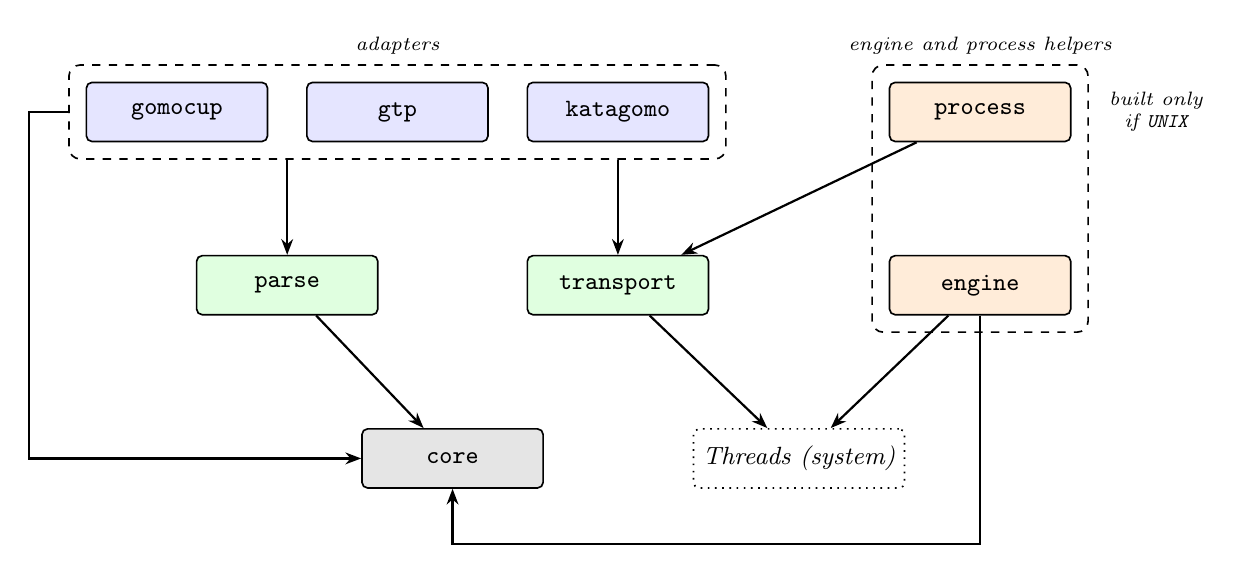
\begin{tikzpicture}[pg figure]
  % Row 1: the adapters (grouped) and the process transport (a helper).
  \node[pg mod=layeradapter] (gomocup) at (0,0)   {gomocup};
  \node[pg mod=layeradapter] (gtp)     at (2.8,0) {gtp};
  \node[pg mod=layeradapter] (kata)    at (5.6,0) {katagomo};
  \node[pg group, fit=(gomocup)(kata), label={[pg note]above:adapters}] (adapters) {};
  \node[pg mod=layerhelper]  (process) at (10.2,0) {process};
  \node[pg note, right=0.35cm of process] {built only\\if \code{UNIX}};
  % Row 2: parse, transport and the engine helpers.
  \node[pg mod=layerio]      (parse)     at (1.4,-2.2)  {parse};
  \node[pg mod=layerio]      (transport) at (5.6,-2.2)  {transport};
  \node[pg mod=layerhelper]  (engine)    at (10.2,-2.2) {engine};
  % Row 3: the core and the system thread library.
  \node[pg mod=layercore]    (core)    at (3.5,-4.4) {core};
  \node[pg ext]              (threads) at (7.9,-4.4) {Threads (system)};
  \node[pg group, fit=(process)(engine), label={[pg note]above:engine and process helpers}]
    (helpers) {};

  \draw[pg arrow] (adapters.south -| parse)     -- (parse);
  \draw[pg arrow] (adapters.south -| transport) -- (transport);
  \draw[pg arrow] (adapters.west) -- ++(-0.5,0) |- (core.west);
  \draw[pg arrow] (process) -- (transport);
  \draw[pg arrow] (parse) -- (core);
  \draw[pg arrow] (transport) -- (threads);
  \draw[pg arrow] (engine) -- (threads);
  \draw[pg arrow] (engine.south) -- ++(0,-2.9) -| (core.south);
\end{tikzpicture}
\caption{Module dependencies: an arrow points from a target to a target it links
  (\code{target\_link\_libraries} in the root \file{CMakeLists.txt}). The arrows leaving the
  dashed adapters box hold for each of the three adapters. The core links nothing, and the
  transport does not link the core. The dashed boxes group the adapters and the engine and process
  helpers; the box shade repeats the layer (core, adapters, parse and transport, helpers) and
  carries nothing else.}
\label{fig:modules}
\end{figure}

\begin{center}
\small
\begin{tabularx}{\textwidth}{@{}>{\ttfamily}l >{\ttfamily}l X@{}}
\toprule
\normalfont\textbf{Target} & \normalfont\textbf{Links} & \textbf{Role} \\
\midrule
gomo\_core      & --- & Neutral types and the \code{EnginePort} / \code{CommandPort} /
                          \code{EventSink} interfaces. No I/O, no threads, no protocol names. \\
gomo\_transport & Threads & \code{Transport} port and \code{StreamTransport}. Protocol-blind;
                          independent of the core. \\
gomo\_parse     & core & Pure text-to-event parsers (Gomocup, GTP) and the \code{LineParser} hook. \\
gomo\_engine    & core, Threads & Blocking \code{search()} and \code{DeadlineEngine}; works
                          with any adapter. \\
gomo\_gomocup   & core, parse, transport & Gomocup adapter and its \code{gomo::encode} builders. \\
gomo\_gtp       & core, parse, transport & GTP adapter (KataGomo extensions) and builders. \\
gomo\_katagomo  & core, parse, transport & KataGomo \code{gom} mode adapter and builders. \\
gomo\_process   & transport & \code{ProcessTransport}: spawns the engine (POSIX only). \\
\bottomrule
\end{tabularx}
\end{center}

\subsection{Rules that are enforced}

\file{scripts/check-core-deps.sh} checks the first two rules; review and the sizing rules
(Section~\ref{sec:process}) hold the other two.

\begin{enumerate}
  \item \textbf{The core is protocol- and I/O-free.} \file{include/gomo/core/} and
        \file{src/core/} include no stream, thread, process, signal or filesystem header, and no
        header whose path names a protocol or engine (\code{gomocup}, \code{gtp}, \code{rapfi},
        \code{katagomo}, \code{transport}, \code{adapter}, \ldots). Checked by
        \file{scripts/check-core-deps.sh}.
  \item \textbf{The transport port is protocol-blind.} \file{include/gomo/transport/} never
        mentions a protocol or engine name. Same script.
  \item \textbf{Adapters never depend on each other.} A new protocol adds a module; it does not edit
        an existing one.
  \item \textbf{Moving a module boundary or adding a cross-layer dependency is a size~L change}: it
        needs an approved planning, then an ADR (Section~\ref{sec:process}).
\end{enumerate}

\subsection{Data flow of one search}

Figure~\ref{fig:search-flow} follows one Gomocup search from the call to the move, with time
running down.

\begin{figure}[tbp]
\centering
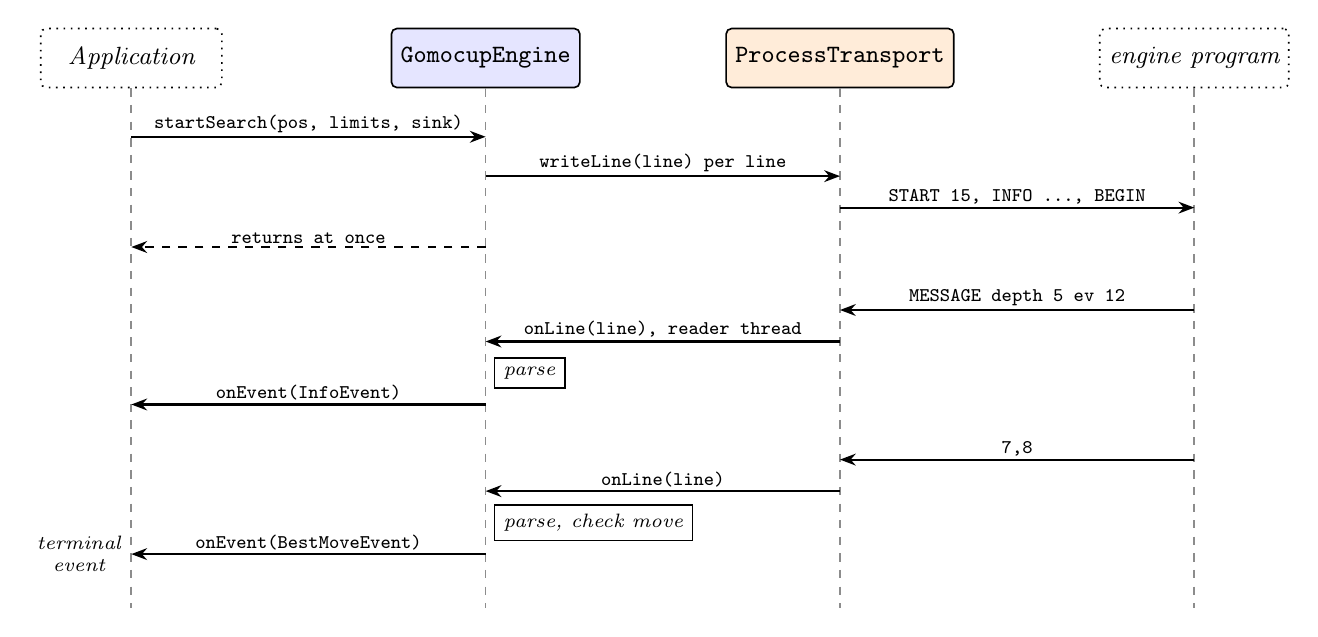
\begin{tikzpicture}[pg figure]
  \node[pg ext]                 (app) at (0,0)    {Application};
  \node[pg mod=layeradapter]    (ad)  at (4.5,0)  {GomocupEngine};
  \node[pg mod=layerhelper]     (tr)  at (9.0,0)  {ProcessTransport};
  \node[pg ext]                 (en)  at (13.5,0) {engine program};
  \foreach \n in {app,ad,tr,en} \draw[pg lifeline] (\n.south) -- ++(0,-6.6);

  \draw[pg arrow] (0,-1.0) -- node[pg label,above]{startSearch(pos, limits, sink)} (4.5,-1.0);
  \draw[pg arrow] (4.5,-1.5) -- node[pg label,above]{writeLine(line) per line} (9.0,-1.5);
  \draw[pg arrow] (9.0,-1.9) -- node[pg label,above]{START 15, INFO ..., BEGIN} (13.5,-1.9);
  \draw[pg arrow, dashed] (4.5,-2.4) -- node[pg label,above]{returns at once} (0,-2.4);
  \draw[pg arrow] (13.5,-3.2) -- node[pg label,above]{MESSAGE depth 5 ev 12} (9.0,-3.2);
  \draw[pg arrow] (9.0,-3.6) -- node[pg label,above]{onLine(line), reader thread} (4.5,-3.6);
  \node[pg note, fill=white, draw, anchor=west] at (4.6,-4.0) {parse};
  \draw[pg arrow] (4.5,-4.4) -- node[pg label,above]{onEvent(InfoEvent)} (0,-4.4);
  \draw[pg arrow] (13.5,-5.1) -- node[pg label,above]{7,8} (9.0,-5.1);
  \draw[pg arrow] (9.0,-5.5) -- node[pg label,above]{onLine(line)} (4.5,-5.5);
  \node[pg note, fill=white, draw, anchor=west] at (4.6,-5.9) {parse, check move};
  \draw[pg arrow] (4.5,-6.3) -- node[pg label,above]{onEvent(BestMoveEvent)} (0,-6.3)
    node[pg note, anchor=east] {terminal\\event};
\end{tikzpicture}
\caption{One Gomocup search. \code{startSearch} writes one line per request line through
  \code{Transport::writeLine} (\code{START}, the \code{INFO} lines, then \code{BEGIN} or
  \code{BOARD}~\ldots~\code{DONE}) and returns before the engine answers. Every later step runs on
  the transport's reader thread: \code{TransportListener::onLine}, the parser, and
  \code{EventSink::onEvent}. Dotted boxes are outside libgomo.}
\label{fig:search-flow}
\end{figure}

\noindent \code{startSearch} writes the request and returns. The transport's reader thread delivers
each line to the adapter (\code{TransportListener::onLine}); the adapter parses it, checks it against
the position, and forwards a \code{SearchEvent} to the caller's \code{EventSink}. The search ends with
exactly one terminal event.


\subsection{Why deadlines live in a decorator}\label{sec:why-deadline}

An engine can stop answering. Something must then end the search, and it must also stop a late
answer from being read as the reply to the next search. Gomocup has no request ids, and Rapfi
ignores synchronising commands while it thinks, so after a timeout the only safe state is
``this engine still owes an answer''.

Two places could own that logic. Putting it in each adapter would repeat a timer, a thread and the
owed-answer state three times, and would give the core's one-search-at-a-time rule a different
timeout story per protocol. libgomo instead wraps any \code{EnginePort} in \code{DeadlineEngine},
so the adapters stay free of timers and threads and every protocol gets the same behaviour
(\file{docs/audit/AUD-03}, which supersedes AUD-01). The price is one more object to create and a
destruction order to respect (Section~\ref{sec:deadline}).

%######################################################################
\part{How-to guides}
%######################################################################

%======================================================================
\section{Using the library}
%======================================================================

\subsection{Linking}

libgomo has no install step yet: add the checkout with \code{add\_subdirectory}, then link the
alias targets you need. Include directories and C++23 come with them.

\begin{lstlisting}[style=sh]
add_subdirectory("/path/to/libgomo" gomo)
target_link_libraries(my_app PRIVATE gomo::gomocup gomo::process gomo::engine)
\end{lstlisting}

\subsection{A blocking search with a deadline}\label{sec:howto-search}

This program runs one search with a deadline. It starts the engine as a child process, speaks
Gomocup to it, and wraps the adapter in \code{DeadlineEngine}. It is the program of
Section~\ref{sec:first} and was compiled and run against a real Rapfi.

\begin{lstlisting}
#include <chrono>
#include <cstdio>
#include <variant>

#include "gomo/engine/blocking_search.hpp"
#include "gomo/engine/deadline_engine.hpp"
#include "gomo/gomocup/gomocup_engine.hpp"
#include "gomo/process/process_transport.hpp"

using namespace gomo;
using namespace std::chrono_literals;

// Plays one search on a 15x15 Renju board and prints the result.
int playOne(EnginePort& engine) {
    if (!engine.setRules(Rules{.board = BoardRule::Renju})) return 1;

    auto position = Position::create(15, 15);
    if (!position || !position->play({7, 7}) || !position->play({8, 7})) return 1;

    auto outcome = search(engine, *position, Limits{.turnTime = 1000ms});
    if (!outcome) {
        std::fprintf(stderr, "search refused: %d\n", static_cast<int>(outcome.error()));
        return 1;
    }
    for (const InfoEvent& info : outcome->info) {
        if (info.depth) std::printf("depth %d\n", *info.depth);
    }
    if (auto* best = std::get_if<BestMoveEvent>(&outcome->terminal)) {
        std::printf("best move %d,%d\n", best->coord.x, best->coord.y);
        return 0;
    }
    if (auto* error = std::get_if<ErrorEvent>(&outcome->terminal)) {
        std::fprintf(stderr, "engine error: %s\n", error->message.c_str());
    }
    return 1;
}

int main(int argc, char** argv) {
    if (argc < 2) return 2;
    ProcessTransport transport{ProcessOptions{.program = argv[1]}};
    GomocupEngine    gomocup{transport};
    DeadlineEngine   engine{gomocup};  // gives every search a turnTime + grace deadline

    const int rc = gomocup.open() ? playOne(engine) : 1;
    // Close before the locals are destroyed (in reverse order): DeadlineEngine must not
    // outlive the stream of events from the reader thread.
    transport.close();
    return rc;
}
\end{lstlisting}

\noindent Points to notice:
\begin{itemize}
  \item \code{playOne} takes an \code{EnginePort\&}, so it works unchanged with \code{GtpEngine}
        or \code{KataGomoEngine}.
  \item Call \code{open()} on the adapter, not on the decorator: \code{open()} is not part of the
        port.
  \item \textbf{Close the transport before the end of scope.} Locals are destroyed in reverse
        order, so the decorator goes first. \code{transport.close()} stops event delivery and
        reaps the child, so no event reaches the destroyed decorator.
\end{itemize}

\subsection{An asynchronous search with a custom sink}

For a GUI or an analysis view, implement \code{EventSink} and react to events as they arrive.
This program streams KataGomo analysis through \code{GtpEngine}. Link \code{gomo::gtp} and
\code{gomo::process} when building it. The example was run against a fake GTP engine.

\begin{lstlisting}
#include <chrono>
#include <condition_variable>
#include <cstdio>
#include <mutex>
#include <type_traits>
#include <variant>

#include "gomo/gtp/gtp_engine.hpp"
#include "gomo/process/process_transport.hpp"

using namespace gomo;
using namespace std::chrono_literals;

// Prints progress as it arrives and wakes waitDone() on the terminal event.
class PrintingSink final : public EventSink {
public:
    void onEvent(const SearchEvent& event) override {  // runs on the reader thread
        std::visit(
            [&](const auto& e) {
                using T = std::decay_t<decltype(e)>;
                if constexpr (std::is_same_v<T, InfoEvent>) {
                    for (const Candidate& c : e.candidates) {  // one GTP line = one snapshot
                        if (c.move && c.visits) {
                            std::printf("%d,%d visits %lld\n", c.move->x, c.move->y,
                                        static_cast<long long>(*c.visits));
                        }
                    }
                } else if constexpr (std::is_same_v<T, MessageEvent>) {
                    std::printf("engine says: %s\n", e.text.c_str());
                } else if constexpr (std::is_same_v<T, UnparsedEvent>) {
                    std::printf("unparsed: %s\n", e.line.c_str());
                } else {
                    if constexpr (std::is_same_v<T, BestMoveEvent>) {
                        std::printf("best move %d,%d\n", e.coord.x, e.coord.y);
                    }
                    std::lock_guard lock(mutex_);
                    done_ = true;
                    cv_.notify_all();
                }
            },
            event);
    }

    void waitDone() {
        std::unique_lock lock(mutex_);
        cv_.wait(lock, [&] { return done_; });
    }

private:
    std::mutex              mutex_;
    std::condition_variable cv_;
    bool                    done_{false};
};

int main(int argc, char** argv) {
    if (argc < 2) return 2;
    ProcessTransport transport{ProcessOptions{.program = argv[1], .args = {"gtp"}}};
    // A real KataGomo also needs its -model and -config arguments here.
    GtpEngine        engine{transport};
    PrintingSink     sink;  // declared after the engine, so it is destroyed first: close first

    int  rc       = 1;
    auto position = Position::create(15, 15);
    if (engine.open() && position) {
        engine.setAnalyze(200ms);  // stream kata-genmove_analyze info lines
        if (engine.startSearch(*position, Limits{.maxNodes = 400}, sink)) {
            sink.waitDone();
            rc = 0;
        }
    }
    transport.close();
    return rc;
}
\end{lstlisting}

\subsection{Practical rules for applications}

Follow these rules in any application built on the port:

\begin{itemize}
  \item Check \code{supports(rules)} or the result of \code{setRules} before a game; an
        unsupported request sends nothing.
  \item Treat \code{InfoEvent} and \code{Candidate} fields as optional. Engines print different
        subsets.
  \item Read the summary for ``how is the search going'' and \code{candidates} for per-move
        analysis. Do not take \code{nodes} as one move's visits, or a candidate's
        \code{visits} as the search total (Section~\ref{sec:candidates}).
  \item Keep \code{UnparsedEvent} and \code{MessageEvent} visible in logs: they are how a new engine
        output format shows up.
  \item Give every search a \code{turnTime}, and wrap the adapter in \code{DeadlineEngine} unless
        you trust the engine to answer.
  \item Return from \code{onEvent} quickly; hand the event to your own queue or thread.
  \item Use \code{sendRaw} for a one-off engine-only line (Rapfi database commands, KataGomo
        \code{kata-set-param} keys). Nothing about the reply is promised; on GTP it never ends a
        search (Section~\ref{sec:limits}). For a command you send often, or whose reply you need,
        use \code{CommandPort} (Section~\ref{sec:own}).
\end{itemize}

%======================================================================
\section{Extending libgomo}
%======================================================================

\subsection{Adding a protocol adapter}

A new protocol is a new module; the core and existing adapters do not change.

\begin{enumerate}
  \item \textbf{Size it.} A new protocol touches a protocol and a public interface: it is a size~L
        change and starts with a planning in \file{features/<slug>/planning.md}
        (Section~\ref{sec:process}).
  \item \textbf{Collect evidence.} Capture real engine transcripts (or, if impossible, derive them
        from the engine's source and label the fixture as source-derived) into
        \file{tests/fixtures/<protocol>/}.
  \item \textbf{Write the parser} in \file{src/parse/} with its header in
        \file{include/gomo/parse/}: pure, total, \code{std::string\_view} and
        \code{std::from\_chars}, no \code{std::regex}. Unknown input becomes \code{UnparsedEvent}.
        Reuse an existing parser if the output format matches (as \code{KataGomoEngine} reuses the
        Gomocup parser).
  \item \textbf{Write the adapter} in \file{include/gomo/<protocol>/} and \file{src/<protocol>/},
        following the shared pattern below.
  \item \textbf{Add the CMake target} \code{gomo\_<protocol>} with alias
        \code{gomo::<protocol>}, linking only \code{gomo::core}, \code{gomo::parse} and
        \code{gomo::transport}; call \code{gomo\_enable\_warnings}.
  \item \textbf{Test} with a fake transport (Section~\ref{sec:testing}), register every test group in
        \file{tests/CMakeLists.txt}, and add a \code{DeadlineEngine} test over the new adapter.
\end{enumerate}

\noindent The adapter pattern every existing adapter follows:

\begin{lstlisting}
class MyEngine final : public EnginePort, private TransportListener {
public:
    explicit MyEngine(Transport& transport) : transport_(transport) {}
    std::expected<void, EngineError> open() {
        if (!transport_.start(*this)) return std::unexpected(EngineError::NotReady);
        return {};
    }
    std::expected<void, EngineError> startSearch(const Position& position, const Limits& limits,
                                                 EventSink& sink) override {
        // 1. Reject what the protocol cannot express, before anything is sent.
        // 2. Under the lock: NotReady if closed_, Busy if sink_; build every line;
        //    set sink_ = &sink and remember the position.
        // 3. Outside the lock: write the lines. On failure, if sink_ is gone the search
        //    already ended (closed mid-start): return success. Else clear sink_, return
        //    TransportFailed.
    }

private:
    void onLine(std::string_view line) override {
        SearchEvent event = parse::parseMyLine(line);
        EventSink*  sink  = nullptr;
        {
            std::lock_guard lock(mutex_);
            sink = sink_;
            if (!sink) return;              // nothing is running: drop the line
            // Check a best move against position_ (on the board, not occupied).
            if (isTerminal(event)) sink_ = nullptr;  // exactly one terminal event
        }
        sink->onEvent(event);               // never call the sink under the lock
    }
    void onClosed(CloseReason) override {
        // Under the lock: closed_ = true, take and clear sink_.
        // Outside it: sink->onEvent(ErrorEvent{"engine connection closed"}) if one was running.
    }

    Transport&              transport_;
    std::mutex              mutex_;
    Rules                   rules_{};
    bool                    closed_{false};
    EventSink*              sink_{nullptr};  // non-null while a search runs
    std::optional<Position> position_;
};
\end{lstlisting}

\noindent Keep timers and threads out of the adapter; \code{DeadlineEngine} owns deadlines
(Section~\ref{sec:why-deadline}).

\subsection{Adding a transport}

Implement \code{Transport}: deliver lines on your own reader thread, serialise listener calls,
call \code{onClosed} exactly once, reject lines containing a newline, bound the line length, and keep
\code{close()} idempotent. Keep protocol and engine names out of
\file{include/gomo/transport/} (checked by \file{scripts/check-core-deps.sh}). A Windows process
transport would be a new module next to \code{gomo\_process}.

\subsection{Adding an event or a core field}

Changing \code{SearchEvent}, \code{EnginePort} or any core type changes a public interface used by
every adapter and application: it is size~L. Precedent: \code{MessageEvent} and \code{ResignEvent}
were added under the planning \file{features/core-message-resign-events/planning.md};
\code{InfoEvent::candidates} under \file{features/detailed-search-analysis/planning.md}, recorded
in ADR-01. The terminal test is one function, \code{isTerminal(const SearchEvent\&)} in
\file{search\_event.hpp}: Info, Message, Unparsed and Custom do not end a search, every other
type does. A new type is terminal unless you add it to that function, so decide there first
(\file{docs/adr/ADR-02-\allowbreak extensible-engine-commands.md}). For output only one application understands,
do not add a type: use \code{CustomEvent} from a \code{LineParser} (Section~\ref{sec:own}). Keep
the variant protocol-neutral, and update every adapter, both parsers and \code{search()} in the
same planning.

%======================================================================
\section{Write your own commands, rules and board layouts}\label{sec:own}
%======================================================================

An engine often has more than the three adapters know: its own output lines, its own rules, walls
on the board, commands that start an analysis. libgomo does not ship these. It gives you five
places to plug them in, and every one is opt-in: set nothing and the adapters behave as before.
The decision and the rejected options are in \file{docs/adr/ADR-02-\allowbreak extensible-engine-commands.md}.

\begin{center}
\small
\begin{tabularx}{\textwidth}{@{}X >{\ttfamily}l X@{}}
\toprule
\textbf{You want to\ldots} & \normalfont\textbf{Use} & \textbf{Where it goes} \\
\midrule
read an output line the parser does not know & LineParser & adapter constructor \\
send a different script for a search (new \code{INFO} lines, another position command) &
  RequestEncoder & adapter constructor \\
ask for a rule the enums lack (Caro) & Rules::extensions & \code{setRules}; read by your encoder \\
describe walls, a torus or portals & BoardLayout & \code{Position::create}; read by your encoder \\
send a command outside a search (an option, an analysis) & CommandPort & \code{execute} on the
  adapter \\
\bottomrule
\end{tabularx}
\end{center}

\noindent The example below drives a made-up Rapfi-like engine (the ``fake Rapfi''). Its lines are
invented for the guide; the commands follow what \file{docs/audit/AUD-08} read in Rapfi's source.
The code was compiled and run against a fake transport.

\subsection{Step 1: read a new output line}

A \code{LineParser} turns one line into one \code{SearchEvent}. Return \code{UnparsedEvent} for any
line that is not yours, and chain your parser before the default one with
\code{parse::chainParsers}. Output only your application understands goes in a
\code{CustomEvent}: a tag and an ordered list of typed fields. It never ends a search.

\begin{lstlisting}
// Reads the fake engine's `VC win 7,7 depth 9` line; anything else stays Unparsed.
SearchEvent parseVcLine(std::string_view line) {
    const std::string text{line};  // sscanf needs a terminated string
    int               x = 0, y = 0, depth = 0;
    if (std::sscanf(text.c_str(), "VC win %d,%d depth %d", &x, &y, &depth) != 3) {
        return UnparsedEvent{text};
    }
    return CustomEvent{.tag    = "vc-win",
                       .fields = {{"move", Coord{x, y}}, {"depth", std::int64_t{depth}}}};
}
\end{lstlisting}

\noindent The parser runs on the transport's reader thread, outside the adapter's lock: it must
not block. It must also never turn a line that ends a search (a move, \code{SWAP}, a fatal
\code{ERROR}) into a non-terminal event, because the adapter trusts \code{isTerminal} of what you
return. On GTP your parser sees the body lines of a reply and free text, not the reply header, and
only a reply ends the search: a parser that swallows the final \code{play X} of an analyze reply
loses the move.

\subsection{Step 2: send your own script}

A \code{RequestEncoder} turns a \code{SearchRequest} (\code{rules}, \code{position},
\code{limits}) into the full list of lines for one \code{startSearch}. You can write every line
yourself, or call the default builder and edit its result. The default builders refuse
\code{Rules::extensions} and a non-default \code{BoardLayout} with \code{Unsupported}, so the
encoder below hands the default a plain request and adds the extras itself:

\begin{lstlisting}
// Sends Caro, torus, walls and portals the way the fake engine wants them.
EncodedRequest fakeRapfiRequest(const SearchRequest& request) {
    // Let the default script write START, the INFO limits and rule; it refuses what it does not
    // know (extensions, layout), so give it a plain request on an empty board.
    auto empty = Position::create(request.position.width(), request.position.height());
    if (!empty) return std::unexpected(EngineError::Unsupported);
    SearchRequest plain{.rules = request.rules, .position = *empty, .limits = request.limits};
    plain.rules.extensions.clear();

    EncodedRequest script = encode::defaultGomocupRequest(plain);
    if (!script) return script;
    script->pop_back();  // the default ends in BEGIN: we send a position block instead

    const BoardLayout& layout = request.position.layout();
    if (request.rules.extensions.contains("caro")) script->push_back("INFO RULE 8");
    if (layout.torus) script->push_back("INFO TORUS 1");
    for (const auto& [a, b] : layout.portals) {
        script->push_back(std::format("INFO YXPORTAL {},{} {},{}", a.x, a.y, b.x, b.y));
    }
    // A position block replaces the walls, so INFO WALL lines would be wiped: the walls go in
    // the block itself, as `x,y,3` entries.
    std::vector<std::string> walls;
    for (const Coord& c : layout.blocked) walls.push_back(std::format("{},{},3", c.x, c.y));
    auto block = encode::boardBlock("BOARD", request.position.moves(), walls);
    script->insert(script->end(), block.begin(), block.end());
    return script;
}
\end{lstlisting}

\noindent \code{encode::boardBlock(command, moves, extra)} writes \code{command}, one
\code{x,y,c} line per move (\code{c} is 1 for the side that moves next, 2 for the other side), the
\code{extra} lines as given, and \code{DONE}. Pass \code{"YXBOARD"} instead of \code{"BOARD"} for
a block that only sets the position and starts no search. Every block, \code{YXBOARD} too, replaces
the engine's walls with its own \code{c=3} entries, so walls belong in the block. Rules for an encoder:

\begin{itemize}
  \item It runs under the adapter's lock. It must be pure, must not block and must not call back
        into the adapter.
  \item Return an error (normally \code{EngineError::Unsupported}) to refuse; then nothing is
        sent.
  \item With an encoder set, \code{supports(rules)} accepts any valid rules: only your encoder
        knows what it can send, and it refuses in \code{startSearch}.
  \item \code{GtpEngine} wants one command per line, no id, one reply each; the last line asks for
        the move. \code{KataGomoEngine} takes any script.
\end{itemize}

\subsection{Step 3: ask for a rule and a layout}

Neither type needs code in the library. A rule the enums lack goes in \code{Rules::extensions},
board structure in a \code{BoardLayout}; the encoder above reads both.

\begin{lstlisting}
Rules rules{.board = BoardRule::Freestyle, .extensions = {{"caro", true}}};
auto  position = Position::create(15, 15, BoardLayout{.torus   = true,
                                                      .blocked = {{3, 3}},
                                                      .portals = {{{1, 1}, {12, 12}}}});
if (!position) return 1;       // OutOfBounds: a wall or portal end is off the board
if (auto ok = position->play({3, 3}); !ok) { /* PositionError::Blocked */ }
if (auto ok = position->play({7, 7}); !ok) return 1;  // walls are not moves: sideToMove() holds
\end{lstlisting}

\noindent The core stores the layout as data and checks only that every cell is on the board.
Whether the engine can play it (torus size, portals on a rectangle) is the engine's call: it
answers with \code{ERROR}. Without your encoder, \code{setRules} refuses the extension and
\code{startSearch} refuses the layout with \code{Unsupported}, and nothing is sent.

\subsection{Step 4: send a command}

\code{CommandPort} sits beside \code{EnginePort}; \code{GomocupEngine}, \code{KataGomoEngine} and
\code{DeadlineEngine} implement it. A \code{Command} is data, and its \code{completion} says how
the adapter knows it is finished:

\begin{center}
\small
\begin{tabularx}{\textwidth}{@{}>{\ttfamily}l X@{}}
\toprule
\normalfont\textbf{Completion} & \textbf{Meaning} \\
\midrule
None   & Done once the lines are written. The sink gets no event. \\
Search & A search: ends with its terminal event; Busy until then. \\
Until  & Ends at the first event for which \code{done(event)} is true; that event still reaches
         the sink. \\
\bottomrule
\end{tabularx}
\end{center}

\begin{lstlisting}
// Fire and forget: INFO VCTHREAD 2
Command vcThread{.name = "INFO", .args = {std::string{"VCTHREAD"}, std::int64_t{2}}};

// A multi-line analysis: YXANALZ, one x,y per line, DONE. It runs as a search.
Command analyze{.name       = "YXANALZ",
                .block      = {Coord{7, 7}, Coord{8, 8}},
                .terminator = "DONE",
                .completion = Command::Search{}};

if (!engine.execute(vcThread, sink)) { /* Busy, NotReady, Unsupported, TransportFailed */ }
auto sent = engine.execute(analyze, sink, CommandOptions{.force = true});
\end{lstlisting}

\noindent \code{commandLines(command)} gives the exact lines (\code{YXANALZ}, \code{7,7},
\code{8,8}, \code{DONE}); \code{format(Value)} is how each argument and block element is written.
Without \code{force}, \code{execute} returns \code{Busy} while a search or a \code{Search} or
\code{Until} command runs, and sends nothing. With \code{force} the adapter stops the running work
(\code{YXSTOP} for Gomocup), queues the command, and returns at once. Rapfi silently drops every
command but \code{STOP} while it thinks, so the command is written only after the old terminal
event has reached its own sink; the old output is not lost. One command can wait; a second
\code{force} returns \code{Busy}.

\subsection{Step 5: wire it together}

\begin{lstlisting}
ProcessTransport transport{ProcessOptions{.program = "fake-rapfi"}};
GomocupEngine    gomocup{transport, parse::chainParsers(parseVcLine, parse::parseGomocupLine),
                         fakeRapfiRequest};
DeadlineEngine   engine{gomocup};  // forwards execute() to gomocup, adds search deadlines
\end{lstlisting}

\noindent Call \code{open()} on the adapter, then \code{setRules}, \code{startSearch} and
\code{execute} on \code{engine}; \code{DeadlineEngine} is both an \code{EnginePort} and a
\code{CommandPort}. In your sink, test for \code{CustomEvent} with \code{std::get\_if} like any
other event type.

\subsection{Limits to know}

\begin{itemize}
  \item \textbf{Completion by \code{Until} can wait forever.} Rapfi has no terminator line for a
        one-shot reply: it is a fixed number of lines, one \code{OK} or \code{ERROR}, or nothing.
        Use \code{None} for a silent command, or bound the wait with \code{DeadlineEngine}.
  \item \textbf{A command has no deadline} (it has no \code{Limits}). Bound a \code{Search}
        command with \code{stop()}, or use \code{Until}.
  \item \textbf{Rapfi V3 can drop a command sent right after its move}, and leaves its arguments
        in the input, where they run as commands. V2 and V3 also differ: \code{YXANALZ} exists
        only in V2, and a list with no valid move ends with a bare \code{ERROR}, which does not
        end a \code{Search} (use \code{Until}). Choose the commands for your engine version.
  \item \textbf{GTP supports \code{None} only.} \code{GtpEngine::canExecute} is false for
        \code{Search}, \code{Until}, a \code{block} or a \code{terminator}. With \code{force}
        during a search it waits for the natural end: \code{stop()} cannot interrupt
        \code{genmove}.
  \item \textbf{Non-square boards.} \code{GomocupEngine}'s default script sends
        \code{RECTSTART w,h}; an engine that does not know it prints \code{ERROR}, which does not
        end a search, so wrap the adapter in \code{DeadlineEngine}. \code{KataGomoEngine} refuses
        them.
\end{itemize}

%======================================================================
\section{Writing and registering tests}\label{sec:testing}
%======================================================================

\subsection{Naming and registering test cases}

A test case name starts with \code{<group>\_<behaviour>:} followed by the behaviour in words, e.g.\
\code{TEST\_CASE("gomo\_stop: YXSTOP is sent and the following move is delivered")}. Each ctest entry
selects cases by that prefix:

\begin{lstlisting}[style=sh]
foreach(group sequence rules events warning stop closed rect deadline)
  add_test(NAME gomo_${group} COMMAND gomo_gomocup_tests "-tc=gomo_${group}*")
endforeach()
\end{lstlisting}

\noindent \textbf{A new prefix needs its own \code{add\_test}}, or the case is built and silently never
run. This happened once (fix-log entry \code{GTP-04-01}); since then
\file{scripts/check-ctest-coverage.sh} (ctest entry \code{ctest\_coverage}) fails when any doctest
case is matched by no ctest filter.

\subsection{Fakes, fixtures and live tests}

The project provides four kinds of test support:

\begin{itemize}
  \item \textbf{Fake transport.} Adapter tests use a \code{FakeTransport} that records written lines
        and lets the test ``play the engine'' by calling \code{listener->onLine(...)} and
        \code{onClosed(...)} directly, so the test checks the exact protocol text without a
        process.
  \item \textbf{Fixtures.} \file{tests/fixtures/gomocup/} holds Rapfi output in its brief, normal and
        UCI-like formats; \file{tests/fixtures/gtp/} holds analysis lines. A fixture derived from
        source rather than captured says so in its header comment.
  \item \textbf{Live tests} need a real engine: set \code{GOMO\_RAPFI} to the
        \code{pbrain-rapfi} executable. Without it every live test prints \code{SKIPPED} and
        ctest reports it as skipped, not passed.
  \item \textbf{ThreadSanitizer.} Adapters, transports and \code{DeadlineEngine} are concurrent; run
        the \code{tsan} preset after touching any of them.
\end{itemize}


%######################################################################
\part{Reference}
%######################################################################

%======================================================================
\section{The core model}
%======================================================================

All core types live in namespace \code{gomo} under \file{include/gomo/core/}. Errors are
returned as \code{std::expected<T, E>}; nothing in the library throws on purpose.

\subsection{Coordinates and moves (\file{coord.hpp}, \file{side.hpp})}

\code{Coord\{x, y\}} is 0-based with the origin at the \emph{top-left}; $x$ grows to the right and
$y$ grows down. Every adapter converts to and from its protocol's notation (for example GTP's
\code{H8}, whose rows count from the bottom); the core never sees protocol notation.
\code{Move\{coord, side\}} is one stone; \code{Side} is \code{Black} (moves first) or \code{White},
and \code{opposite(side)} returns the other one.

\subsection{Position (\file{position.hpp})}

\code{Position} holds a board size and the moves played, in order:

\begin{lstlisting}
auto position = Position::create(15, 15);   // expected<Position, PositionError>
if (!position) { /* InvalidBoardSize: outside 1..Position::kMaxSide (1024); OutOfBounds:
                    a cell of the optional BoardLayout argument is off the board */ }
if (auto ok = position->play({7, 7}); !ok) { /* OutOfBounds, Blocked or Occupied; unchanged */ }
position->sideToMove();   // Black after an even number of moves
position->moves();        // span<const Move>, in the order played
\end{lstlisting}

\noindent A position is any rectangle; whether an engine accepts a non-square board is the
adapter's decision (Gomocup and GTP do, \code{KataGomoEngine} does not). \code{Position} knows
nothing about wins or forbidden moves: it records stones and rejects only off-board, blocked or
occupied points, checked in that order. A third argument, \code{BoardLayout}, adds structure
without changing the moves: \code{torus}, \code{blocked} cells (WALL), \code{portals} (cell
pairs) and free-form \code{extensions}. \code{layout()} returns it, \code{blocked(c)} asks about
one cell, and \code{==} compares it. The core checks only that every cell is on the board; torus
size, portals on a rectangle and similar limits are the engine's to refuse.

\subsection{Rules (\file{rules.hpp})}

\code{Rules\{board, opening, maxMoves, extensions\}}. \code{BoardRule} is \code{Freestyle} (five or more wins),
\code{Standard} (exactly five) or \code{Renju}. \code{OpeningRule} is \code{FreeOpen},
\code{Swap1} or \code{Swap2}. Board and opening rules are separate fields; an adapter whose
protocol needs one combined rule number (Gomocup) builds it. \code{validate(rules)} checks
self-consistency
(\code{maxMoves} must be positive); \code{EnginePort::supports(rules)} says whether an engine can play
them. \code{extensions} is a \code{std::map<std::string, Value>} for rules the enums do not model
(Caro); an adapter without a custom encoder refuses a non-empty map.

\subsection{Limits (\file{limits.hpp})}

\code{Limits\{turnTime, matchTime, maxDepth, maxNodes\}}; every field is optional. An empty field
means ``no limit from the caller'' and the engine applies its own default. An adapter that cannot
express a set field returns \code{Unsupported} and sends nothing.

\subsection{Search events (\file{search\_event.hpp})}

Everything an adapter reports during a search is one \code{SearchEvent}:

\begin{lstlisting}
using SearchEvent = std::variant<InfoEvent, BestMoveEvent, SwapEvent, PassEvent, ResignEvent,
                                 ErrorEvent, MessageEvent, UnparsedEvent, CustomEvent>;
\end{lstlisting}

\begin{center}
\small
\begin{tabularx}{\textwidth}{@{}>{\ttfamily}l c X@{}}
\toprule
\normalfont\textbf{Event} & \textbf{Terminal} & \textbf{Meaning} \\
\midrule
InfoEvent     & no  & Progress: an optional summary (\code{depth}, \code{nodes}, \code{score},
                      \code{elapsed}, \code{principalVariation}) and a list of \code{candidates}.
                      Engines differ in what they print. \\
BestMoveEvent & yes & The engine's chosen move (already checked to be on the board and free). \\
SwapEvent     & yes & The engine swaps sides in a swap opening. \\
PassEvent     & yes & The engine passed. Gomoku has no pass; callers may treat it as an error. \\
ResignEvent   & yes & The engine resigned. \\
ErrorEvent    & yes & The search failed: fatal engine error, illegal move, closed connection, or
                      timeout. \code{message} is for humans, not for parsing. \\
MessageEvent  & no  & Free text the engine sent on purpose (e.g.\ Gomocup \code{MESSAGE}). \\
UnparsedEvent & no  & A line no parser understood, kept whole. \\
CustomEvent   & no  & Output only an application's own parser understands: a \code{tag} and
                      typed \code{fields} (\code{Value}). \\
\bottomrule
\end{tabularx}
\end{center}

\noindent \code{isTerminal(event)} is the single test for the Terminal column; adapters,
\code{search()} and \code{DeadlineEngine} all call it. \code{Value} is a closed variant of
\code{bool}, \code{std::int64\_t}, \code{double}, \code{std::string}, \code{Coord}, \code{Move}
and vectors of the last two; \code{format(Value)} gives its default wire text.

\noindent \code{Score} has a \code{kind} (\code{Eval}, \code{MateIn}, \code{MatedIn}) and a
\code{value}, always from the side to move's point of view.

\paragraph{Summary and candidates.}\label{sec:candidates} An \code{InfoEvent} carries two views
of a report (ADR-01, \file{docs/adr/ADR-01-info-event-candidates.md}):

\begin{itemize}
  \item \textbf{The summary} describes the search as a whole. \code{depth} and \code{elapsed} are
        of the whole search. \code{nodes} is only the search total, never the visits of one move.
        \code{score} and \code{principalVariation} come only from an unranked line or the
        rank-1 candidate; a report about the second-best move leaves them empty.
  \item \textbf{\code{candidates}} is a \code{std::vector<Candidate>}, one entry per move the
        report describes, in printed order. Every field of a \code{Candidate} is optional:
        \code{rank} (1 = best, only when the engine prints one), \code{move}, \code{score},
        \code{visits} (spent on this move only), \code{winrate} and \code{drawrate} (both
        $0..1$), and the \code{principalVariation} starting with this move.
\end{itemize}

\noindent How the two protocols fill it:

\begin{center}
\small
\begin{tabularx}{\textwidth}{@{}l X X@{}}
\toprule
 & \textbf{Gomocup (Rapfi)} & \textbf{GTP analysis (KataGomo)} \\
\midrule
One report    & One line per candidate: a ranked line gives one \code{Candidate}; unranked
                lines (\code{depth ... pv}, \code{Speed ...}, \code{Bestline}) give none.
              & One line holds every candidate: each \code{info} entry is one
                \code{Candidate}, so a line is a whole snapshot. \\
\code{rank}   & \code{(N)} or \code{multipv N}. & \code{order k} gives $k+1$; empty without
                \code{order}. \\
\code{visits} & \code{V} / \code{v}. & \code{visits}. \\
Win / draw    & \code{W}/\code{D} or \code{w}/\code{d} percentages, divided by 100.
              & \code{winrate} only: $0..1$ when the entry has \code{utility}
                (\code{kata-analyze}), else divided by 10000 (\code{lz-analyze}). No draw rate. \\
Summary       & \code{nodes} from \code{n}, \code{Node} or the \code{Speed} line's
                \code{Visit}; \code{score} and PV from unranked or rank-1 lines.
              & \code{nodes} and \code{score} empty; PV from rank 1, or from the first entry
                when no entry has \code{order}. \\
\bottomrule
\end{tabularx}
\end{center}

\noindent A rate outside $0..1$ is left empty. The framework never groups Gomocup lines into
snapshots: it cannot know where one search iteration ends, so the application groups ranked
lines itself (for example, a new \code{rank == 1} starts a new set).

%======================================================================
\section{The engine port}\label{sec:port}
%======================================================================

\code{EnginePort} (\file{core/engine\_port.hpp}) is the only interface an application needs.

\begin{lstlisting}
class EnginePort {
public:
    virtual bool supports(const Rules& rules) const = 0;
    virtual std::expected<void, EngineError> setRules(const Rules& rules) = 0;
    virtual std::expected<void, EngineError> startSearch(
        const Position& position, const Limits& limits, EventSink& sink) = 0;
    virtual void stop() = 0;
    virtual std::expected<void, EngineError> sendRaw(std::string_view line) = 0;
};

class EventSink {
public:
    virtual void onEvent(const SearchEvent& event) = 0;
};
\end{lstlisting}

\subsection{Contract}

Every adapter keeps these promises; tests in \file{tests/core/engine\_port\_test.cpp} and the
adapter suites check them.

\begin{enumerate}
  \item \textbf{A refused call sends nothing.} \code{setRules} and \code{startSearch} validate
        first; on \code{Unsupported} not a byte reaches the engine.
  \item \textbf{Non-blocking start.} \code{startSearch} writes the request and returns. It does not
        wait for the engine.
  \item \textbf{Exactly one terminal event per started search}: best move, swap, pass, resign or
        error. A closed connection during a search produces
        \code{ErrorEvent\{"engine connection closed"\}}.
  \item \textbf{One search at a time.} A second \code{startSearch} while one runs returns
        \code{Busy}.
  \item \textbf{The sink is called on the adapter's thread} (the transport's reader thread), in
        arrival order, never concurrently with itself, and \emph{never while the adapter holds a
        lock}. The sink may therefore call back into the port, for example to start the next
        search from inside the terminal event.
  \item \textbf{The sink must outlive the search} and must not block for long: it holds up reading
        the engine's output.
  \item \textbf{\code{stop()} is a request.} It may be called from any thread and is harmless when
        no search runs. If the protocol cannot interrupt a search, the search runs to its own end;
        the terminal event still arrives.
  \item \textbf{\code{sendRaw} promises nothing.} Replies arrive as ordinary events (usually
        \code{MessageEvent} or \code{UnparsedEvent}) while a search runs; outside a search they
        are dropped.
\end{enumerate}

\subsection{Errors}

A refused call returns one of these \code{EngineError} values:

\begin{center}
\small
\begin{tabularx}{\textwidth}{@{}>{\ttfamily}l X@{}}
\toprule
\normalfont\textbf{EngineError} & \textbf{Returned when} \\
\midrule
Unsupported     & The rules, position or limits cannot be expressed in the protocol. Nothing sent. \\
Busy            & A search is already running (or, under \code{DeadlineEngine}, a timed-out search
                  still owes its answer). \\
NotReady        & The adapter is not open (\code{open()} failed) or its connection closed. \\
TransportFailed & Writing a line to the engine failed. \\
\bottomrule
\end{tabularx}
\end{center}

%======================================================================
\section{Transports}
%======================================================================

\subsection{The port (\file{transport/transport.hpp})}

A \code{Transport} is a full-duplex, line-oriented text channel. It knows nothing about what the
lines mean.

\begin{itemize}
  \item \code{start(listener)} begins delivering received lines to a \code{TransportListener}
        (\code{onLine(line)}, then \code{onClosed(reason)} exactly once).
  \item \code{writeLine(line)} sends one line; the transport adds the terminator. A line that
        contains \code{\textbackslash n} is rejected with \code{InvalidLine}, so framing cannot
        break. Safe from any thread.
  \item \code{close()} is idempotent; afterwards \code{writeLine} fails with \code{Closed} and the
        listener gets no further lines.
\end{itemize}

\noindent \code{CloseReason}: \code{Eof}, \code{Requested}, \code{LineTooLong}, \code{IoError}.
\code{TransportError}: \code{NotStarted}, \code{AlreadyStarted}, \code{Closed}, \code{InvalidLine},
\code{IoError}. Both implementations strip a trailing \code{\textbackslash r}, deliver empty
lines, deliver a final line without newline at end of input, and end the transport with
\code{LineTooLong} when a line exceeds \code{maxLineLength} (default 1\,MiB), so a misbehaving engine
cannot exhaust memory.

\subsection{ProcessTransport (POSIX)}

\code{ProcessTransport} spawns the engine and uses its stdin and stdout as the channel. Its
options and their defaults:

\begin{lstlisting}
ProcessOptions options;
options.program          = "pbrain-rapfi";   // looked up in PATH when it has no '/'
options.args             = {};
options.workingDirectory = "";               // empty: inherit
options.mergeStderr      = false;            // false: the child's stderr goes to /dev/null
options.maxLineLength    = 1U << 20;
options.grace            = std::chrono::milliseconds{400};
ProcessTransport transport{options};
\end{lstlisting}

\begin{itemize}
  \item \textbf{Start.} A missing program is reported by \code{start()} as \code{IoError}.
  \item \textbf{Closing.} \code{close()} wakes the reader, closes the child's stdin, waits
        \code{grace}, sends \code{SIGTERM}, waits again, then \code{SIGKILL}, and reaps the child.
        From another thread it returns after that; from inside the listener it returns at once and
        the cleanup finishes on the reader thread. \code{onClosed} runs after the child is reaped,
        so \code{exitStatus()} is valid inside it (exit code, or $-N$ for signal $N$).
  \item \textbf{Process group.} The child runs in its own process group, which is killed when the
        child ends, so helper processes die with it. A process that calls \code{setsid} escapes.
        Ctrl-C at the terminal does not reach the child.
  \item \textbf{SIGPIPE} is blocked only on the writing thread inside \code{writeLine}; the
        process-wide disposition is never changed. Writing to a dead child returns \code{IoError}.
\end{itemize}

\subsection{StreamTransport}

\code{StreamTransport} wraps an already connected \code{std::istream}/\code{std::ostream} pair,
which it does not own. It suits sockets and tests. A read blocked inside the input stream cannot
be interrupted: \code{close()}
silences the listener and stops writing at once, but the reader thread ends only when the stream
reaches end of input or fails, and the destructor waits for that. Whoever owns the pipe or socket
must close it.

%======================================================================
\section{Protocol adapters}
%======================================================================

All three adapters share one shape: they implement \code{EnginePort} and \code{CommandPort},
privately implement \code{TransportListener}, do not own the transport (it must outlive them),
and need one call to \code{open()} before use. Each constructor takes the transport and two
optional hooks, a \code{LineParser} and a \code{RequestEncoder}; empty means the built-in one
(Section~\ref{sec:own}). \code{setRules} only stores the rules; \code{startSearch} sends
everything, including the full position, each time.

\subsection{Capability matrix}

What each adapter can express and how it reports results:

\begin{center}
\small
\begin{tabularx}{\textwidth}{@{}l X X X@{}}
\toprule
 & \textbf{GomocupEngine} & \textbf{GtpEngine} & \textbf{KataGomoEngine} \\
\midrule
Reference engine     & Rapfi (run live) & KataGomo \code{gtp} (source only) &
                       KataGomo \code{gom} (source only) \\
Board                & any rectangle (\code{RECTSTART w,h} when not square) & any rectangle up to
                       625 columns & square only \\
Board rules          & all three & all three & all three \\
Swap1 / Swap2        & freestyle only & no & no \\
\code{maxMoves}      & yes & yes & yes \\
\code{turnTime}      & yes & yes (\code{maxTime}) & yes \\
\code{matchTime}     & yes & Unsupported & Unsupported \\
\code{maxDepth}      & yes & Unsupported & Unsupported \\
\code{maxNodes}      & yes & yes (\code{maxVisits}) & yes (\code{maxVisits}) \\
\code{stop()}        & sends \code{YXSTOP} & no-op & no-op \\
\code{ERROR} line    & \code{MessageEvent}; search continues & \code{?} reply ends search &
                       terminal \code{ErrorEvent} \\
Streaming info       & \code{MESSAGE} lines & with \code{setAnalyze()} & \code{MESSAGE} lines as
                       \code{MessageEvent} \\
Swap / pass / resign & \code{SwapEvent} & \code{PassEvent}, \code{ResignEvent} & \code{SwapEvent} \\
\code{CommandPort}  & \code{None}, \code{Search}, \code{Until}; \code{force} sends \code{YXSTOP}
                       & \code{None} only; \code{force} waits for the search to end
                       & \code{None}, \code{Search}, \code{Until}; \code{force} waits \\
Extension types      & custom parser and encoder & custom parser and encoder & custom parser
                       and encoder \\
\bottomrule
\end{tabularx}
\end{center}

\subsection{GomocupEngine}

\code{GomocupEngine} speaks Gomocup with Yixin extensions. For each search, \code{startSearch}
sends:

\begin{lstlisting}[style=sh]
START 15                    # RECTSTART 15,10 for a non-square board
INFO rule 4                 # 0 freestyle, 1 standard, 4 renju, 5 swap1, 6 swap2
INFO max_moves 225          # only for the fields that are set
INFO timeout_turn 1000
INFO timeout_match 60000
INFO max_depth 20
INFO max_node 1000000
BOARD                       # or BEGIN for an empty board
7,7,2                       # x,y,owner: 1 = side to move, 2 = opponent
8,7,1
7,8,2
DONE
\end{lstlisting}

\noindent This is the default script (\code{encode::defaultGomocupRequest}); a custom
\code{RequestEncoder} replaces it. Replies are parsed by \code{parse::parseGomocupLine} unless you
pass a \code{LineParser}. An \code{ERROR} line during a search
is \emph{not} the end: Rapfi prints non-fatal errors and still answers, so it becomes a
\code{MessageEvent} and the search waits for a move. A returned move that is off the board or on an
occupied point becomes \code{ErrorEvent\{"engine returned an illegal move: ..."\}}. Lines outside a
search (banners, late replies) are dropped. The adapter has no timer: if the engine never answers,
the search stays open until the transport closes, unless \code{DeadlineEngine} wraps the adapter.

\subsection{GtpEngine}

\code{GtpEngine} speaks GTP with KataGomo's Gomoku extensions. For each search it sends these
commands, each with a numeric id:

\begin{lstlisting}[style=sh]
1 boardsize 15 15
2 clear_board
3 RENJU                       # FREESTYLE / STANDARD / RENJU
4 maxmoves 225
5 kata-set-param maxTime 1.000
6 kata-set-param maxVisits 400
7 play B H8                   # every move, in order
8 play W J8
9 genmove B                   # or: kata-genmove_analyze B interval 20
\end{lstlisting}

\begin{itemize}
  \item \textbf{Reply framing.} A header \code{=id body} or \code{?id body}, then body lines, then a
        blank line. Replies are matched to commands by order: the reply to a \code{sendRaw} line
        becomes \code{MessageEvent} during a search and never ends it (AUD-04). The rules below
        are for replies to the search's own commands. Replies with an id outside the running
        search are ignored (stale replies of an earlier search). A \code{?} reply ends the search
        with \code{ErrorEvent}.
  \item \textbf{Result.} The \code{genmove} reply becomes \code{BestMoveEvent}, \code{PassEvent}
        (\code{pass}) or \code{ResignEvent} (\code{resign}). An occupied point, an unreadable
        move, an analysis reply without a final \code{play}, and a reply without an id each end
        the search with \code{ErrorEvent}.
  \item \textbf{Analysis.} \code{setAnalyze(interval)} switches later searches to
        \code{kata-genmove\_analyze}: the engine streams \code{info} lines before the final
        \code{play X}. Each line is one \code{InfoEvent} whose \code{candidates} hold every entry
        of the line (Section~\ref{sec:candidates}). The interval is rounded down to
        centiseconds, minimum 1.
  \item \textbf{Free text} outside a reply during a search becomes a \code{MessageEvent}; outside a
        search it is dropped.
  \item \textbf{stop() is a no-op.} KataGomo reads stdin on one thread, so a line sent during
        \code{genmove} is read only after the move is chosen (\file{docs/audit/AUD-02}). Searches
        are bounded by the limits sent before them.
\end{itemize}

\noindent Vertices: columns \code{A..Z} skipping \code{I}, two letters from column 25; rows count
from the bottom. Letters cover at most 625 columns, so on a wider board \code{startSearch} returns
\code{Unsupported} for any position with moves. The parser also reads the machine form
\code{(x,y)} (0-based, origin top-left); the adapter never sends it. See
\code{parse::parseGtpVertex} and \code{formatGtpVertex}.

\subsection{KataGomoEngine (\code{gom} mode)}

\code{KataGomoEngine} drives KataGomo's \code{gom} mode, which mixes GTP-style rule commands with
Gomocup position commands. For each search it sends:

\begin{lstlisting}[style=sh]
START 15                      # resets the board, so the settings follow it
RENJU
maxmoves 225
INFO timeout_turn 1000
kata-set-param maxVisits 400
BOARD                         # colours alternate from Black; an empty list is the empty board
7,7
8,7
DONE
\end{lstlisting}

\noindent The engine's \code{OK} reply to \code{START} is ignored. Output is parsed with the Gomocup
parser; unlike \code{GomocupEngine}, an \code{ERROR} line here ends the search with an
\code{ErrorEvent}. The engine only reads \code{time\_left} and \code{timeout\_turn} from \code{INFO};
rules come from the rule commands.

\subsection{Parsers}

Parsers live in namespace \code{gomo::parse}, are pure and total, and never throw.

\begin{description}[style=nextline]
  \item[\code{parseGomocupLine(line)}] \code{SWAP} $\to$ \code{SwapEvent};
    \code{ERROR text} $\to$ \code{ErrorEvent}; \code{x,y} $\to$ \code{BestMoveEvent};
    \code{MESSAGE ...} $\to$ \code{InfoEvent} when it has an info shape, else \code{MessageEvent};
    anything else $\to$ \code{UnparsedEvent}. Info shapes understood:
    \begin{itemize}
      \item UCI-like: \code{depth 10-12 ev 34 n 1.2M tm 900 pv 7,7 8,8} (the first token must be
            \code{depth} or \code{multipv}, so prose is never mistaken for info);
      \item Rapfi normal and brief: \code{Speed 333K | Depth 5-6 | Eval -67 | Node 373 | Time 1ms},
            optional \code{[Pondering]} prefix, MCTS \code{Visit}, multi-PV \code{(1) 34 | 5-6 | E5 B2},
            and \code{Bestline H7 J9 I9}.
    \end{itemize}
    A ranked line (\code{(N) ...} or \code{multipv N ...}) gives one \code{Candidate}; only
    rank~1 fills the summary \code{score} and PV (Section~\ref{sec:candidates}).
    Counts accept \code{K/M/G/T} suffixes; scores accept \code{+M<n>}/\code{-M<n>} (mate). In
    the Rapfi shapes \code{Time} accepts \code{ms}, \code{s}, \code{min} and \code{h}; in the
    UCI-like shape \code{tm} is plain milliseconds. Labels like \code{H8} in a PV mean column
    letter and 1-based row counted from the top, with \code{A1} = \code{(0,0)}.
  \item[\code{parseGtpResponseHeader(line)}] \code{=}/\code{?}, optional id (at most 9 digits), body.
  \item[\code{parseGtpVertex(text, w, h)} / \code{formatGtpVertex(coord, w, h)}] vertex conversion.
  \item[\code{parseGtpAnalyzeLine(line, w, h)}] a \code{kata-analyze} / \code{lz-analyze}
    \code{info} line; every entry becomes a \code{Candidate}. A broken first entry gives
    \code{UnparsedEvent}; a broken later entry keeps the candidates before it. Score fields are
    not read (in KataGomo Gom2026 they hold the draw rate), nor are \code{prior}, \code{lcb} and
    \code{utility}.
\end{description}

\noindent \code{parseGomocupLine} does not know the board size; the adapter checks each returned
move. The GTP vertex functions take the board size and reject points outside it.

%======================================================================
\section{Engine helpers}
%======================================================================

\subsection{Blocking search (\file{engine/blocking\_search.hpp})}

\code{search()} runs one search and collects its events:

\begin{lstlisting}
struct SearchOutcome {
    std::vector<InfoEvent>   info;      // progress reports, in arrival order
    std::vector<SearchEvent> other;     // MessageEvent and UnparsedEvent
    SearchEvent              terminal;  // BestMove, Swap, Pass, Resign or Error
};
std::expected<SearchOutcome, EngineError> search(
    EnginePort& engine, const Position& position, const Limits& limits);
\end{lstlisting}

\noindent \code{search()} uses only \code{startSearch}, so it works with every adapter. It blocks
until the terminal event: if the engine never answers, it never returns, unless
\code{DeadlineEngine} wraps the adapter. Do not call it from the thread that delivers events (for
example from inside a sink).

\subsection{DeadlineEngine (\file{engine/deadline\_engine.hpp})}\label{sec:deadline}

\code{DeadlineEngine} is a decorator that gives any \code{EnginePort} a search deadline. It is the
only place with timeouts; adapters have no timers (\file{docs/audit/AUD-03}).
Figure~\ref{fig:deadline} shows the timeline of a search that times out.

\begin{figure}[tbp]
\centering
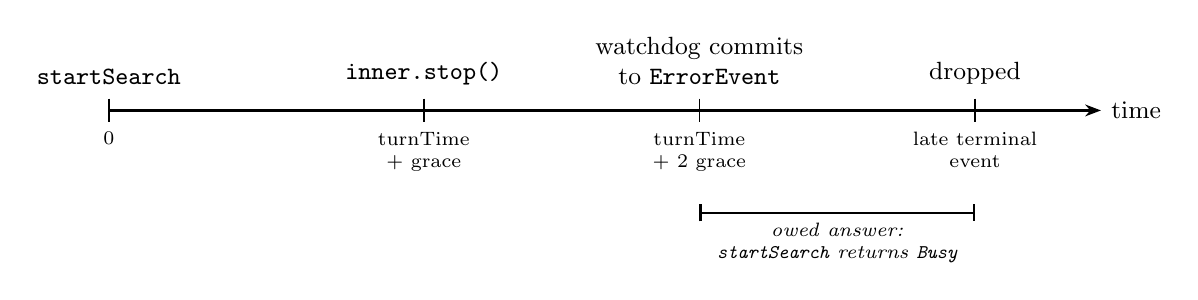
\begin{tikzpicture}[pg figure]
  \draw[pg arrow] (0,0) -- (12.6,0) node[right] {time};
  \foreach \x/\t in {0/{0},
                     4/{turnTime\\+ grace},
                     7.5/{turnTime\\+ 2 grace},
                     11/{late terminal\\event}} {
    \draw (\x,0.15) -- (\x,-0.15) node[below, pg note, font=\scriptsize] {\t};
  }
  \node[above, align=center] at (0,0.2)   {\code{startSearch}};
  \node[above, align=center] at (4,0.2)   {\code{inner.stop()}};
  \node[above, align=center] at (7.5,0.2) {watchdog commits\\to \code{ErrorEvent}};
  \node[above, align=center] at (11,0.2)  {dropped};
  \draw[line width=0.8pt, {Bar}-{Bar}] (7.5,-1.3) -- (11,-1.3)
    node[midway, below, pg note] {owed answer:\\\code{startSearch} returns \code{Busy}};
\end{tikzpicture}
\caption{A search that times out in \code{DeadlineEngine}. Only a search with
  \code{Limits::turnTime} $> 0$ has a deadline. A terminal event that arrives before
  \code{turnTime + 2 grace}, even after \code{stop()}, ends the search normally and cancels the
  deadline. After the watchdog commits to the error, it waits for any active callback to return.
  The decorator refuses new searches until it begins the timeout callback and drops the late
  terminal event. If that event never arrives, the decorator stays \code{Busy} and the caller
  must close the transport
  (\file{docs/audit/AUD-03}).}
\label{fig:deadline}
\end{figure}

\begin{itemize}
  \item Only a search with \code{Limits::turnTime} $> 0$ gets a deadline; \code{grace} defaults to
        2000\,ms (\code{DeadlineEngine::Options}).
  \item At \code{turnTime + grace} the decorator calls \code{stop()} on the wrapped port. After one
        more \code{grace} the watchdog schedules \code{ErrorEvent\{"engine did not answer"\}}
        and drops further events from that search.
  \item The watchdog starts the timeout callback once active callbacks from that search have
        returned. It calls the sink with the state mutex unlocked, so the sink can call
        \code{startSearch}. That call returns \code{Busy} while timeout delivery is pending or
        the engine still owes its answer (Section~\ref{sec:why-deadline}).
  \item If the engine never answers, the decorator stays \code{Busy}; close the transport.
  \item \textbf{Commands.} \code{DeadlineEngine} is also a \code{CommandPort}: \code{execute}
        forwards to the wrapped engine, or returns \code{Unsupported} if it is not one. A command
        has no deadline. With \code{force} over a search of this object, the command is kept and
        sent after that search's terminal event; if the search times out instead, it is never sent
        and its sink gets an \code{ErrorEvent}, because the engine may still be thinking.
  \item \textbf{Lifetime.} Keep the sink alive until the terminal callback returns. The wrapped
        port must outlive the decorator. Close the transport and let the wrapped port finish
        delivering events before destroying the decorator.
\end{itemize}

%======================================================================
\section{Test map}\label{sec:testmap}
%======================================================================

Each module has one doctest executable; two more cover \code{DeadlineEngine} over the GTP and
KataGomo adapters, and the live Rapfi tests. All of them share \file{tests/main.cpp}. The smoke
test is a plain program without doctest. Names below omit the \code{gomo\_} prefix.

\begin{center}
\footnotesize
\begin{tabularx}{\textwidth}{@{}>{\ttfamily}l X >{\raggedright\arraybackslash\ttfamily}X@{}}
\toprule
\normalfont\textbf{Executable} & \textbf{Covers} & \normalfont\textbf{ctest entries} \\
\midrule
core\_tests     & Coord, Position (with layout), Rules, Limits, events, \code{Value}, port
                          contract, \code{CommandPort} &
                          core\_tests, port\_sink, port\_contract, ext01\_*, ext02\_core,
                          ext05\_core, ext06\_core \\
transport\_tests & StreamTransport & transport\_\{lines, write, close, limit, misc\} \\
parse\_tests    & Gomocup and GTP parsers, fixtures & parse\_*, gomo2\_parse, gomo2\_fixtures, gtp\_* \\
engine\_tests   & search(), DeadlineEngine & port\_blocking, dead1\_* \\
gomocup\_tests  & GomocupEngine (fake transport) & gomo\_* \\
gtp\_tests      & GtpEngine (fake transport) & gtp2\_*, gtp3\_*, gtp4\_message, gtp5\_text \\
katagomo\_tests & KataGomoEngine (fake transport) & kata\_* \\
deadline\_adapter\_tests & DeadlineEngine over GTP and KataGomo & dead2\_\{gtp, kata\} \\
process\_tests  & ProcessTransport (POSIX) & proc\_* \\
live\_tests     & GomocupEngine against real Rapfi & gomo2\_\{live, stop, close, deadline\} \\
smoke           & core links, one short game & smoke \\
\bottomrule
\end{tabularx}
\end{center}

\noindent The \code{ext*} entries cover the extension points, one prefix per todo of the planning
(\code{ext02} to \code{ext10}: custom event, parser, rules, layout, encoder, rectangular boards,
\code{CommandPort}) in each adapter's executable, plus \code{ext09\_live} against Rapfi V3 (skipped
without \code{GOMO\_RAPFI\_V3}).

\noindent Plus three script checks registered as ctest entries: \code{ctest\_coverage},
\code{style\_line\_length} and \code{style\_doc\_comments}.


%######################################################################
\part{Contributing}
%######################################################################

%======================================================================
\section{Coding style}
%======================================================================

The full rule is \file{.claude/rules/coding-style.md}. The essentials:

\begin{itemize}
  \item C++23, 4-space indent, types \code{PascalCase}, functions \code{camelCase}, members with a
        trailing underscore. Match the surrounding code; never restyle a file you are only editing.
  \item \textbf{100 columns} at most (ctest entry \code{style\_line\_length}).
  \item \textbf{Errors as values}: \code{std::expected} and an error enum per layer; mark fallible
        calls \code{[[nodiscard]]}.
  \item \textbf{Doc comments}: every public type, function and method in \file{include/} has a
        \code{///} comment directly above it; struct and enum members get a trailing
        \code{///<}. The first sentence is a third-person summary. Then only what the signature
        does not say: units, errors, ownership and lifetime, thread-safety, blocking. Checked by
        \code{style\_doc\_comments}.
  \item In \file{src/}, comment the \emph{why}: a protocol quirk, a lock-ordering constraint, a
        workaround, with the spec section, audit or todo id when there is one. No commented-out
        code. TODOs have an owner: \code{TODO(owner): action}.
  \item \textbf{clang-format owns the layout.} Run \code{clang-format -i} on the files you change;
        the pinned config \file{.clang-format} sets alignment, wrapping and include order. The
        ctest entry \code{style\_format} (\file{scripts/check-format.sh}) fails on any file the
        formatter would change.
\end{itemize}

%======================================================================
\section{How work is organised}\label{sec:process}
%======================================================================

The repository records work, decisions and evidence next to the code, in a set of documents and
scripts called the harness. \file{docs/README.md} maps the folders.

\subsection{Sizing}

Decide the size before touching anything. Size comes from risk and ambiguity, not file count; when
unsure, choose the larger size.

\begin{center}
\small
\begin{tabularx}{\textwidth}{@{}l X X X@{}}
\toprule
\textbf{Size} & \textbf{Signal} & \textbf{Documents} & \textbf{Gate before code} \\
\midrule
S & few files, one layer, reversible, no decision & expiring note in \file{docs/notes/} & none \\
M & real work, nothing hard to reverse & todo in \file{docs/todo/} plus its features in
    \file{docs/features.json} & read the todo; audit if a decision was made \\
L & cross-layer, interface, protocol, format, toolchain or process & planning in
    \file{features/<slug>/} $\to$ approved $\to$ todos (each $\leq$ M) $\to$ audit or ADR &
    planning approved, no open questions \\
\bottomrule
\end{tabularx}
\end{center}

\subsection{Todos and acceptance features}

A todo (\file{docs/todo/<DOMAIN>-<NN>-<slug>.md}) is one doable item; its frontmatter
\code{status} (\code{backlog} $\to$ \code{active} $\to$ \code{done} $\to$ \code{archived}) is the
truth, and \file{TODO.md} is a generated index. Acceptance lives in \file{docs/features.json}: one
entry per check, written as WHEN/THEN, with a \code{checked\_by} command and a \code{passes} flag. A
todo is done only when all its features pass. Contributors change only \code{passes}, and only after
running \code{checked\_by}; never weaken a check or edit a test to make something pass.

\subsection{Decisions and bugs}

Decisions, bugs and experiments each leave their own record:

\begin{itemize}
  \item \textbf{Audits} (\file{docs/audit/}) record non-bug decisions; \textbf{ADRs}
        (\file{docs/adr/}) record hard-to-reverse architecture decisions. Both are immutable:
        supersede, never edit (AUD-03 supersedes AUD-01).
  \item \textbf{Bugs} follow one chain: reproduce, find the root cause, add a regression check that
        stays, write a \file{docs/fix-log.md} entry. When the first fix was in the wrong layer, the
        entry says so (``First fix'' vs ``Real source'').
  \item \textbf{Spikes} answer ``can this be done?'', are labelled as spikes and thrown away; the
        answer is recorded, not the code (example: AUD-02).
\end{itemize}

\subsection{A session}

A work session follows these steps:

\begin{enumerate}\raggedright
  \item Read \file{docs/handoff.md}, \code{git log --oneline -10}, the active todo
        (\code{node scripts/harness/harness-track.mjs <CODE>}), and run the smoke test.
  \item Work on one feature at a time; verify it the way a user would (real command, real engine
        where possible), then commit with a message that says what changed and why.
  \item Run \code{node scripts/harness/harness-check.mjs} before committing harness documents.
  \item At the end, overwrite \file{docs/handoff.md}: doing now, next step, uncertain points,
        blockers.
\end{enumerate}

%======================================================================
\section{Known limitations}\label{sec:limits}
%======================================================================

What version 0.1.0 does not do, or has not verified against a real engine:

\begin{itemize}
  \item \textbf{Real-engine coverage differs by adapter.} The Gomocup adapter is verified against
        a real Rapfi (live tests, skipped without \code{GOMO\_RAPFI}). The GTP and KataGomo
        adapters were never run against a real engine: their wire format comes from reading
        KataGomo \code{Gom2026} at commit \code{9a0e65c}, and they are tested with fake transports
        only. VCN rules and \code{kata-set-rule} are not mapped.
  \item \textbf{No interruption for GTP or KataGomo}: \code{stop()} is a no-op (AUD-02). Bound the
        search with \code{turnTime} or \code{maxNodes}.
  \item \textbf{An engine that never answers} after a timeout keeps \code{DeadlineEngine} in
        \code{Busy}; the caller must close the transport (AUD-03). The timeout path was run
        against a frozen Rapfi; for GTP and KataGomo only against fake transports.
  \item \textbf{GTP: replies are matched by order.} The adapter tells a raw command's reply from
        a search's by its place in the reply order (\code{MessageEvent} during a search, never the
        end of one; AUD-04). An engine that skips a reply puts every later reply out of step until
        the connection is closed.
  \item \textbf{Lines outside a search are dropped} by every adapter (there is no sink to receive
        them).
  \item \textbf{Not covered by fixtures:} late \code{[Pondering]} lines and Rapfi's
        \code{coord\_conversion\_mode} other than \code{none}, which also swaps the width and height
        in \code{RECTSTART}.
  \item \textbf{Extension points have known gaps} (ADR-02, AUD-08): Rapfi V3 can drop a command sent
        right after its move; \code{Until} cannot complete a command whose success prints nothing;
        the default illegal-move check does not reject a move on a blocked cell;
        \code{BoardLayout} equality depends on the order of its cells, and duplicate walls are
        accepted; the \code{tsan} preset does not build on g++~15 until a separate \code{-Werror}
        failure is fixed.
  \item \textbf{KataGomo \code{MESSAGE Visits ... Winrate ...} lines} are not an info shape the
        Gomocup parser knows; they arrive as \code{MessageEvent}, with no structured fields.
  \item \textbf{Candidate data has limits.} GTP \code{winrate} is from whatever perspective the
        engine reports: KataGomo follows its \code{reportAnalysisWinratesAs} setting (default:
        side to move), which the framework cannot see. GTP has no draw rate, and Gomocup ranked
        lines are not grouped into snapshots. \code{prior}, \code{lcb}, \code{utility},
        \code{seldepth} and \code{stdev} are not kept.
  \item \textbf{ProcessTransport is POSIX-only}; a process that calls \code{setsid} escapes the
        process-group kill.
  \item \textbf{\code{check-doc-comments.sh} is a heuristic}: data members and enumerators are
        reviewed by hand.
\end{itemize}

\subsection*{Further reading in the repository}

\begin{itemize}
  \item \file{features/engine-protocol-port/planning.md} --- the architecture decision (rationale;
        the code is the truth for the wire format).
  \item \file{features/engine-search-deadline/planning.md}, \file{docs/audit/AUD-01..03} ---
        deadlines and the owed answer.
  \item \file{docs/adr/ADR-01-info-event-candidates.md} --- why per-move analysis lives in
        \code{InfoEvent::candidates} (planning:
        \file{features/detailed-search-analysis/planning.md}).
  \item \file{docs/adr/ADR-02-\allowbreak extensible-engine-commands.md} --- why commands, rules, board
        layouts, parsers and encoders are extension points (planning:
        \file{features/\allowbreak extensible-\allowbreak engine-\allowbreak commands/\allowbreak planning.md}; Rapfi facts:
        \file{docs/audit/AUD-08}).
  \item \file{docs/knowledge/} --- background notes (hexagonal style, adapter, strategy, SOLID,
        coupling and cohesion, testability).
  \item \file{docs/fix-log.md} --- root causes of past bugs and the checks that now catch them.
\end{itemize}

\end{document}
